%
% Acta Acustica united with Acustica -- Instructions for Authors, 2017-03-01
%
\documentclass[onecolumn]{article}

%%%%%%%%%%%%%%%%%%%%%%%%%%%%%%%%%%%%%%%%%%%%%%%
%% Comment / uncomment for one or two column(s) fomat
%\documentclass{article}

\usepackage[modulo,switch]{lineno}
\modulolinenumbers[1]
%%%%%%%%%%%%%%%%%%%%%%%%%%%%%%%%%%%%%%%%%%%%%%%
%% Comment / uncomment for showing line numbers

\usepackage[utf8]{inputenc}
\usepackage{amsmath}
\usepackage{wrapfig}
\usepackage{amssymb}
\usepackage{graphicx}
\usepackage{float}
\usepackage{setspace}
\usepackage{enumitem}
\usepackage{titlesec}
\usepackage{lipsum}% just to generate text for the example

\usepackage{listings}
\usepackage{xcolor}

% This is to include code
\usepackage{listings}
\usepackage{xcolor}
\definecolor{dkgreen}{rgb}{0,0.6,0}
\definecolor{gray}{rgb}{0.5,0.5,0.5}
\definecolor{mauve}{rgb}{0.58,0,0.82}
\lstdefinestyle{Python}{
	language        = Python,
	basicstyle      = \ttfamily,
	keywordstyle    = \color{blue},
	keywordstyle    = [2] \color{teal}, % just to check that it works
	stringstyle     = \color{green},
	commentstyle    = \color{red}\ttfamily
}
\lstdefinestyle{PythonWarning}{
	language        = Python,
	basicstyle      = \color{red}\ttfamily,
}

\titlespacing*{\section}
{0pt}{5pt}{5pt}
\titlespacing*{\subsection}
{0pt}{5pt}{5pt}

\makeatletter\@ifundefined{date}{}{\date{}}
\makeatother
\setstretch{1}
\setlist[itemize]{noitemsep}

\paperheight297mm \paperwidth210mm
\textwidth177mm  \textheight290mm  \oddsidemargin 8mm
\evensidemargin\oddsidemargin \hoffset-20mm \voffset-40mm
\topmargin0pt \headheight8mm \headsep2mm \topskip0mm
\footskip7.5mm \columnsep8mm \arraycolsep2pt \parindent5pt
\renewcommand{\abstractname}{Abstract} 

\begin{document}
	
	\title{Project 1: Search}
	
	\author{Franziska Rothen - franziska.rothen@students.unibe.ch - \today}
	
	\maketitle\thispagestyle{empty}
	
	\section{Question 1: Depth First Search}
	
	\begin{wrapfigure}{r}{3.5cm}
		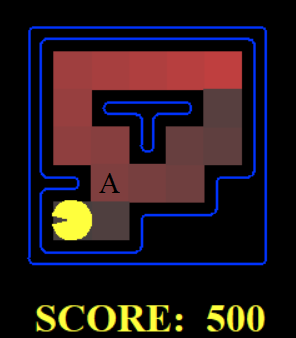
\includegraphics[width=3.5cm]{p1_1.PNG}
		\caption{Example of end state of Pacman in a tiny maze after DFS.}
		\label{fig:p1}
	\end{wrapfigure} 

	With the depth first search method, we choose "the left most" path and follow it as far as possible. When a dead end is reached (end node that is not the goal node), we jump back to the last node with another possible path and continue from there. \newline
	
	In the case seen in figure \ref{fig:p1}, Pacman (starting in the top right corner going in the direction to the left) took a wrong turn at node A and explored the nodes east of it. Once it discovered that this is a dead-end, it jumped back to node A and explored the south (where the goal is found eventually). The path that includes the goal state is saved and given as input of the path for Pacman. Nevertheless, the path in the east was explored and therefore marked red.
	
	For this algorithm, a stack was used. It works with a last-in-first-out (LIFO) queuing policy. The successor states for each node are ordered as follows: 
	\begin{lstlisting}[style=Python]
	[((x, y), 'North', cost), ((x, y), 'South', cost), //
	((x, y), 'East', cost), ((x, y), 'West', cost)]
	\end{lstlisting}
	For the choice of the next node, the stack is popped (starting with the last element), giving the direction the following descending priorities: 'West' - 'East' - 'South' - 'North' 

	This coincides with the decision taken in figure \ref{fig:p1} ('West' over 'South', 'East' over 'South')
		
	\section{Question 2: Breadth First Search}
	The breadth first search explores all the successor states of the starting node and expands evenly in depth. The cost for each step is ignored, resulting in a solution that is possibly not the least cost path.
	
		
	\section{Question 3: Uniform Cost Search}
	
	We explore again each of the successor states of the starting node as in BFS. For further exploration however, the total cost of each following step is calculated. This way we are guaranteed that for each step we follow the path of the lowest cost and finally the goal is reached with the the least cost solution. 
	
		
	\section{Question 4: A* Search}
	On the open maze, the goal was found with the following results for the different search strategies:\newline
	
	\begin{tabular}{|c|c|c|c|}
		\hline
		Strategy & Cost & Speed & Nodes expanded \\ \hline\hline 
		DFS & 298 & 0.3 s & 806 \\  				\hline
		BFS & 54 & 0.1 s & 682 \\ 					\hline
		UCS & 54 & 0.1 s & 682 \\ 					\hline
		A* Search & 54 & 0.1 s & 535\\ 				\hline
	\end{tabular} 
	\newline\newline\newline
	DFS uses the most computational power since it expands the most nodes before finding the goal. This is due to the fact that in the worst case, the DFS will explore the entire search tree before finding the goal. The cost of the winning path is clearly not optimal.\newline
	When comparing BFS and UCS we see that they yield the same results. This can be explained by the fact that the cost of each node is equal, resulting in no improvement from BFS to UCS. \newline
	With the A* Search however, the heuristic function is included in the strategy of choosing the next node. It adds the closest path to the goal from a given state (Manhattan heuristic). This leads to the path never taking a turn that will lead it further away from the goal in the case of an open path.
	
	\section{Question 5: Corner Problem BFS}
	When using an A* search, the algorithm makes sure the exploration is directed towards the missing corner. This means that if a corner has already been found, the heuristic will lead it away from the found corner respectively it will attract it to the corners yet to be explored. this way, the amount of nodes expanded can be minimized.
	
	\newpage
	\vspace*{80px}

	\section{Question 6: Corner Problem A* Search}	
	The most important part of the corners heuristic is to give the states that are closer to a nearby corner a lower heuristic value. This will direct Pacman towards the closest corner. To find the corner with the lowest distance to the current node (whose heuristic is to be determined) the Manhattan distance to each corner was calculated and the lowest value chosen. From there, depending on how many corners are left undiscovered, the total smallest distance to the remaining corners is added.
	Once a corner is detected, it is ignored for the calculation of further heuristic values. This is done in the following way (pseudo-code):
	
	\begin{lstlisting}[style=Python]
	if number_undiscovered_corners == 4:
		distance = manhattan_distance_to_closest_corner + 2 * height + width
	elif number_undiscovered_corners == 3:
		distance = manhattan_distance_to_closest_corner + height + width
	elif number_undiscovered_corners == 2:
		distance = manhattan_distance_to_closest_corner +
		mahattan_distance_to_remaining_corner
	elif number_undiscovered_corners == 1:
		distance = manhattan_distance_to_corner
	\end{lstlisting}
	
	where height and width are the dimensions of the maze, distance is the return value of the heuristic function.

	
	\section{Question 7: Suboptimal Search}
	Fill in foodHeuristic in searchAgents.py with a consistent heuristic for the FoodSearchProblem. Try your agent on the trickySearch board and explain its behaviour

	\section{Question 8: Suboptimal Search}
		
	\begin{wrapfigure}{r}{3.5cm}
		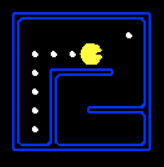
\includegraphics[width=3.5cm]{p8.PNG}
		\caption{Example of suboptimal greedy search.}
		\label{fig:p8}
	\end{wrapfigure} 
	The greedy search won't always find the shortest possible path through the maze. Figure \ref{fig:p8} shows one simple example. Here the total distance to the bottom left corner is clearly further away than the top right which would be the obvious food dot to pick first. But since it is further away form Pacman than the one to its left, it will follow this lead, resulting in a longer path.
	
\end{document}